\documentclass{article}
\usepackage[utf8]{inputenc}
%\usepackage [danish]{babel} % Vi burde ikke have brug for den her
\usepackage[a4paper, hmargin={2.8cm, 2.8cm}, vmargin={2.5cm, 2.5cm}]{geometry}
\usepackage{eso-pic} % \AddToShipoutPicture
\usepackage{graphicx} % \includegraphics
\usepackage{wrapfig, blindtext}
\usepackage{array}
\usepackage{import}
\usepackage[hidelinks]{hyperref}
\usepackage{verbatim}
\usepackage{algorithm}
\usepackage{float}
\linespread{1.2}
\usepackage{pbox}
\usepackage{amsthm}
\usepackage{mathtools}
\usepackage{amsmath}
\usepackage{url}
\usepackage{listings}
\usepackage{tikz}
\usetikzlibrary{arrows,automata,fit}
\usepackage{amsfonts}
\usepackage{standalone}
\newtheorem{theorem}{Teorem}
\newtheorem{lemma}{Lemma}
\newtheorem{korollar}{Korollar}
\newcolumntype{L}[1]{>{\raggedright\let\newline\\\arraybackslash\hspace{0pt}}m{#1}}
\newcolumntype{C}[1]{>{\centering\let\newline\\\arraybackslash\hspace{0pt}}m{#1}}
\newcolumntype{R}[1]{>{\raggedleft\let\newline\\\arraybackslash\hspace{0pt}}m{#1}}

\newcommand*\Let[2]{\State #1 $\gets$ #2}
\usepackage[noend]{algpseudocode}

\usepackage{algorithmicx}

\newtheorem{mydef}{Definition}
\newtheorem{myex}{Example}[section]
\usepackage{caption}
\DeclareMathOperator*{\argmin}{arg\,min}

\author{
\huge{Supervisors}\\
\Large{Rasmus Fonseca}\\
\Large{Niels Bjørn Bugge Grathwohl}\\
\Large{Ulrik Rasmussen}\\
    \\ \texttt{}
}

\title{
  \vspace{3cm}
  \Huge{Genome pattern matching using regular expressions} \\
  \Large{Simon Nicolai Lefoli Maibom - xvm226} \\
  \Large{Arinbjörn Brandsson - hkt789}\\
  \Large{Martin Simon Haugaard - cdl966}
}

\usepackage{natbib}
\usepackage{graphicx}

\newcommand{\myfl}{\left\lfloor}
\newcommand{\myfr}{\right\rfloor}
\newcommand{\mycl}{\left\lceil}
\newcommand{\mycr}{\right\rceil}

\begin{document}

%% Change `ku-farve` to `nat-farve` to use SCIENCE's old colors or
%% `natbio-farve` to use SCIENCE's new colors and logo.
\AddToShipoutPicture*{\put(0,0){\includegraphics*[viewport=0 0 700 600]{lib/natbio-farve}}}
\AddToShipoutPicture*{\put(0,602){\includegraphics*[viewport=0 600 700 1600]{lib/natbio-farve}}}

%% Change `ku-en` to `nat-en` to use the `Faculty of Science` header
\AddToShipoutPicture*{\put(0,0){\includegraphics*{lib/nat-en}}}

\clearpage\maketitle
\thispagestyle{empty}

\newpage
\begin{abstract}
%insert abstract
\end{abstract}
\newpage
\tableofcontents
 
\newpage

%\section{Introduction}
\section{Motivation}
When the human genome project (a project which had the goal of sequencing 
all 22 chromosomes of the human genome) was launched in 1990, the project was 
budgeted to cost 3 billion dollars and was estimated to take fifteen years 
to complete. However as technology progressed, the project managed to complete 
its goal two years earlier than expected, in 2003. This was made possible 
because of the rapid advancements in genome sequencing, and the advancement 
hasn't stopped since. This has lead to decreasing costs of sequencing RNA and DNA, 
meaning biologists has access to greater amounts of data than ever before. 
However the technology to process these amounts of data haven't progressed at 
the same pace as sequencing has. A tool for this is scan\_for\_matches, a 
pattern-matching tool that searches through text files to match a pattern specified 
by a user. While scan\_for\_matches has proven to be a fast and reliable 
tool, because of the amount of data it shifts through, a faster alternative 
is desired.\\\\
After hearing about this problem, we thought that there must be a better 
way of searching through text that is also theoretically sound. Our first 
thought was using automata-based searching methods, since this provides a 
calculable best- and worst-case run time while being theoretically sound. 
Since regular expressions uses an automata-based way of searching, we hypothesized 
that implementing regular expressions that would have the same functions as 
scan\_for\_matches would lead to faster run times.

\section{Problem Analysis}\label{probanal}
%INTRODUCTION TO PROBLEM ANALYSIS
The functionality of scan\_for\_matches dictates what our solution must be able 
to do. While a more indepth analysis of the functionality 
of scan\_for\_matches can be found in Section~\ref{scanformatches}, 
the requirements for our solution are as follows:
\begin{enumerate}
\item Read a data file
\item Match
\begin{enumerate}
\item with mismatches allowed
\item a previously found match
\item a modified pattern
\end{enumerate}
\item Return matches with their position
\end{enumerate}
While some of the functionality (items 1 and 3) will be trivial to implement 
since they are standard functions of most programming languages, there are 
some challenges to be found in regards of what we must match. Matching with 
mismatches allowed are not supported natively in regular expressions, and 
matching a modified text, which may first be determined at runtime, will be 
challenging to implement with automata.

\section{State-of-the-Art}
 \subsection{RE2} %Google's RE engine
 RE2 is Google's regular expression engine written in C++. It supports 
 backtracking, but not backreferencing since backreferencing can't be implemented 
 efficiently according to~\cite{web6}. Since RE2 doesn't support matching with 
 errors or backreferencing, it would be unable to properly reproduce 
 scan\_for\_matches' functionality.
 
 \subsection{TRE} %Got both backtracking and backreferencing
 TRE was created by Ville Laurikari for his master's thesis in 2001, and 
 is a regular expression engine supporting backtracking, backreferencing and 
 matching with errors. Because of this, TRE is the best candidate for modification 
 in order to make it work with patterns. We expand on this in section~\ref{tre}.

%\newpage

%\section{Preliminaries}
\section{Deoxyribonucleic and Ribonucleic Acids}
Deoxyribonucleic acids (DNA) and ribonucleic acids (RNA), collectively known as 
nucleic acids, are one of the three 
essential molecules for life, the last two being proteins and carbohydrates. 
DNA creates RNA through transcription and RNA creates proteins through 
translation, while proteins performs a variety of tasks, one 
of which is packaging and controlling the long DNA molecules~\cite[p. 172]{alberts}. 
In this section we will detail the functions of DNA and RNA as well as their 
secondary structure.
\subsection{DNA}
Deoxyribonucleic acid (DNA) is a macro molecule composed of nitrogenous bases 
joined by deoxyribose-phosphate into long strands. One nitrogenous base which 
is joined with a sugar\footnote{Deoxyribose or ribose}-phosphate is called a 
nucleotide. DNA can have four nitrogenous bases:
\begin{itemize}
\item Guanine (G)
\item Adenine (A)
\item Cytosine (C)
\item Thymine (T)
\end{itemize}
DNA is mostly found in nature as helixes, where two strands have bonded. Each 
base has a complementary base which they can form a hydrogen bond with. 
G is the complementary base of C and A is the complementary base of T.\\\\
DNA holds the hereditary material of the cell and can replicate itself by 
detaching two bonded strands, and use each as a template for a new strand 
to bond with the detached strands~\cite[p. 199]{alberts}.
\subsection{RNA}
Ribonucleic acid (RNA) is a macro molecule composed of long strands of 
nucleotides. RNA have the same nitrogenous bases as DNA except for T, which is 
changed during transcription from DNA to RNA as Uracil (U) which bonds with 
A. In nature, the predominant form of RNA are as a single-stranded chain that 
can fold back on itself or bundled with other chains to form a structure. This 
flexibility of the backbone that allows for the chain to fold in on itself is 
possible because the RNA's backbone is composed of a sugar called ribose, which 
allows more flexibility compared to its other form, deoxyribose, used in 
deoxyribonucleic acid (DNA).\\\\
When DNA creates RNA through transcribing portions of its sequence\footnote{A 
sequence is a succession of nucleotides}, five different kinds of RNA are 
created\cite[p. 236, table 7-1]{alberts}:
\begin{itemize}
\item Messenger RNA (mRNA)
\item Ribosomal RNA (rRNA)
\item Transfer RNA (tRNA)
\item MicroRNAs (miRNA)
\item Other small RNA
\end{itemize}
Where mRNA, rRNA and tRNA are responsible for protein synthesis, while miRNA 
regulates the gene expression of DNA in the cell.
\subsection{Secondary Structure}\label{structs}
The secondary structure of DNA and RNA describes how the bases of the 
strand has bonded to itself. The secondary structure can change if 
the strand is damaged or has mutated, causing it to gain or lose 
bases. Below are examples of three common secondary structures.
\subsubsection{Bulge}
A bulge occurs when one or more bases have no base to bond with, and these 
bases are surrounded by bases that have bonded. This causes the bases to get 
pushed out slightly, resembling a bulging growth. This type of structure occurs 
when one or more bases has been inserted or deleted. If a base has been 
inserted then it will have no base to bond with, and if a base has been deleted 
then the previously-bonded base will have no base to bond with. Figure~\ref{fig:bulge} shows a bulge.

\begin{figure}[H]
\centering
\includegraphics[scale=0.4]{./lib/bulge.png}
\caption{The RNA sequence {\tt AGCAGGCUAGCCGCU}. Note the bulging {\tt A} at position 4.}
\label{fig:bulge}
\end{figure}~
\\
\subsubsection{Interior Loop}
An interior loop is when two or more opposing bases are not complementary and 
can not bond, causing them both to bulge. This occurs when one or more 
consecutive bases mutate to another base. Figure~\ref{fig:int-loop} shows an interior 
loop.
\begin{figure}[h!]
\centering
\includegraphics[scale=0.4]{./lib/interior-loop.png}
\caption{The RNA sequence {\tt AGCAGGCUAGCCGGCU}. Note the bulging {\tt A} at position 4 and {\tt G} at position 13
creating a loop inside the bonded strand.}
\label{fig:int-loop}
\end{figure}\\
These interior loops vary in size, and can have differing amount of bases on 
either side of the strands.
\subsubsection{Stem Loop}
A stem loop, also known as a hairpin loop, occurs when a strand bonds with 
itself, but leaves a sequence of bases sticking out that does not bond with anything. 
This kind of loop occurs typically in RNA as they are single-stranded, but may 
happen in single stranded DNA. Figure~\ref{fig:stem-loop} 
shows a stem loop.
\begin{figure}[h!]\centering
\includegraphics[scale=0.35]{./lib/stem-loop.png}
\caption{A stem loop of the RNA sequence {\tt AAAAUUGGUCUUUU}.}
\label{fig:stem-loop}
\end{figure} 
An important thing to take note of is how the sequence can be seen as one 
long strand that starts from the adenine bases that binds with the uracil bases, 
loops around without binding to anything and finally become the uracil bases 
that the adenine bases from the start binds with. This means that the 
stem loop can be written as one continuous sequence of bases; {\tt AAAAUUGGUCUUUU}. 
Since we can define a stem loop, we can, with the right tools, search through 
a file documenting the bases of a nucleic acid and find all stem loops.


%\section{Theory}
\newpage
\section{Regular expressions} 
  To explain what a regular expression is, we must first introduce languages and alphabets. All literals will be written using the typewriter font, to distinguish 
\begin{mydef}\label{alph}
An alphabet $\Sigma$ is a finite set of letters.
\end{mydef}

\begin{mydef}\label{lang}
A language is a infinite set of strings, composed by letters from an alphabet $\Sigma$
\end{mydef}

\begin{myex}
If we have a DNA sequence string, the alphabet $\Sigma$ consists of the literals ${\tt\{t,g,c,a\}}$. and the language contains strings formed by the literals from this alphabet. For example "gtcaaa" or "gtcaaat". 
\end{myex}

\begin{mydef}
E is a regular expression(RE) if either:
\begin{itemize} 
\item E is a atomic expression, that consist of a letter from an alphabet $\Sigma$ or special character 1.
\item Given two RE's $E_1$ and $E_2$. E is a compound expression formed by $E_1 + E_2$, $E_1 E_2$ or $E_1 ^*$ 
\end{itemize}
\end{mydef}



\begin{mydef}
A regular expression is described by the following grammar: \\
\begin{center}
$E::= a|1|E_1 + E_2 |E_1 E_2 | E^* | 0$
\end{center}
where $E_1$ and $E_2$ are RE's and $a \in \Sigma$
\end{mydef}

\begin{mydef}\centering
The language interpation of L(E) of a regular expression is: 
\begin{align*}
L(0)           &= \emptyset\\
L({\tt a})     &= \{{\tt a}\} \\
L(1)         &= \{\epsilon\} \\
L(E_0 + E_1) &= L(E_0) \cup L(E_1) \\
L(E_1 E_2)   &= \{w_1w_2 | w_1 \in L(E_1),w_2 \in L(E_2)\}=L(E_1)L(E_2) \\
L(E^*)       &= \bigcup\limits_{n=0}^\infty L(E)^n 
\end{align*}
%\cite[p.5 def. 3]{crash}
\end{mydef}

With definition 2, we can now form regular languages. For example, natural numbers described as a regular expression. Natural numbers have the alphabet $\Sigma$ = \{{\tt 0,1,2,3,4,5,6,7,8,9}\}, the regular expression for natural numbers would look like:
\begin{center}
$E_{nat} = $(1+2+3+4+5+6+7+8+9)(0+1+2+3+4+5+6+7+8+9)$^*$
\end{center}

\newpage

\newpage
\section{Nondeterministic Finite Automaton}
\begin{mydef}
An nondeterministic finite automaton (NFA) is a 5-tuple $(Q,\Sigma,\Delta,q^s ,q^a)$. Where $Q$ is a finite set of states,$\Sigma$ is the input alphabet, the initial state $q^s \in Q$,  the accepting state $q^a \in Q$ and $\Delta$ is the set that contains all the transitions. Transitions in $\Delta$ is shown $q^1\xrightarrow{a}q^2$ where $q^1\in Q,q^2\in Q$ and the label $a$ is either $a \in \Sigma$ or  the empty transition $\epsilon$
\end{mydef}

\subsection{Conversion from RE to NFA}
\label{RA_TO_NFA}
One of the main reasons for using NFAs when working with regular expressions is the direct correlation between regular expressions and NFAs. Each expression can be converted to an NFA, and vice versa. Table~\ref{tab:NFA_TAB} shows the correlation between regular expressions and NFA for the most common expressions.
%\\
%(( NOTE: We'll include a table with conversions ))
%\\
%With little effort every regular expression can be translated into a graph, which can then be analysed.

\begin{table}[h]
\caption{Translation table from regular expressions to NFA}
\centering
\begin{tabular}{*{2}{m{0.4\textwidth}}}
\hline
\begin{center}$0$\end{center} &\begin{center}
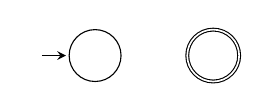
\begin{tikzpicture}[->,>=stealth,shorten >=1pt,auto,node distance=2 cm, scale = 0.75, transform shape,initial text={}]
  \node [initial, state] (0) {};
  \node [accepting,state, right of=0] (1) {};

\end{tikzpicture}\end{center} \\
\hline
\begin{center}$1$\end{center} &\begin{center} 
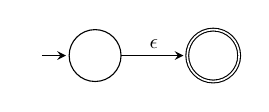
\begin{tikzpicture}[->,>=stealth,shorten >=1pt,auto,node distance=2 cm, scale = 0.75, transform shape,initial text={}]
  \node [initial, state] (0) {};
  \node [accepting,state, right of=0] (1) {};

  \path[->] (0) edge node [above] {$\epsilon$} (1);

\end{tikzpicture} \\
\end{center} \\
\hline
\begin{center}$a$\end{center} &\begin{center} 
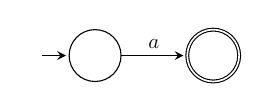
\begin{tikzpicture}[->,>=stealth,shorten >=1pt,auto,node distance=2 cm, scale = 0.75, transform shape,initial text={}]
  \node [initial, state] (0) {};
  \node [accepting,state, right of=0] (1) {};

  \path[->] (0) edge node [above] {$a$} (1);

\end{tikzpicture}\end{center} \\
\hline
\begin{center}$E^1E^2$\end{center} &\begin{center} 
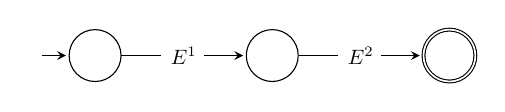
\begin{tikzpicture}[->,>=stealth,shorten >=1pt,auto,node distance=1.5 cm, scale = 0.75, transform shape,initial text={}]
  \node [initial, state] (0) {};
  \node [right of= 0] (1) {$E^1$};
  \node [state,right of= 1] (2) {};
  \node [right of= 2] (3) {$E^2$};
  \node [accepting, state,right of= 3] (4) {};

  \path[-] (0) edge node {} (1);
  \path[-] (2) edge node {} (3);

  \path[->] (1) edge node {} (2);
  \path[->] (3) edge node {} (4);
  
\end{tikzpicture}\end{center} \\
\hline
\begin{center}$E^1 + E^2$\end{center} &\begin{center} 
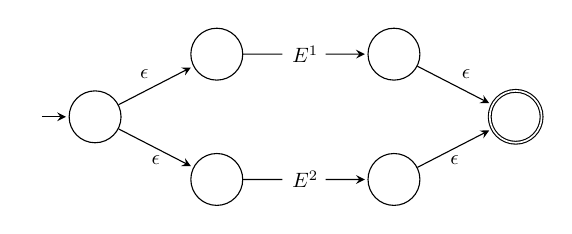
\begin{tikzpicture}[->,>=stealth,shorten >=1pt,auto,node distance=1.5 cm, scale = 0.75, transform shape,initial text={}]
  \node [initial, state] (0) {};
  \node [state,above right of=0,xshift=1cm] (1) {};
  \node [state,below right of=0,xshift=1cm] (2) {};
  \node [right of =1] (3) {$E^1$};
  \node [right of=2] (4) {$E^2$};
  \node [state, right of=3] (5) {};
  \node [state, right of=4] (6) {};
  \node [accepting,state,below right of=5,xshift=1cm] (7) {};

  \path[-] (1)edge node {} (3);
  \path[-] (2)edge node {} (4);

  \path[->] (0) edge node {$\epsilon$} (1);
  \path[->] (0) edge node[below] {$\epsilon$} (2);
  \path[->] (3) edge node {} (5);
  \path[->] (4) edge node {} (6);
  \path[->] (5) edge node {$\epsilon$} (7);
  \path[->] (6) edge node[below] {$\epsilon$} (7);


\end{tikzpicture} \end{center} \\
\hline
\begin{center}$E^*$\end{center} &\begin{center} 
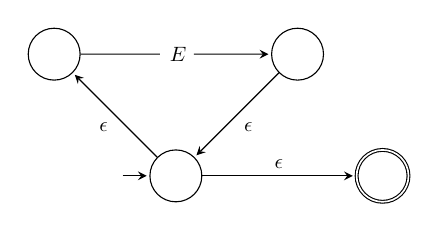
\begin{tikzpicture}[->,>=stealth,shorten >=1pt,auto,node distance=1.5 cm, scale = 0.75, transform shape,initial text={}]
  \node [initial, state] (0) {};
  \node [accepting,state,right of=0,xshift=2cm] (1) {};
  \node [state,above left of=0,xshift=-1cm,yshift=1cm] (2) {};
  \node [state,above right of=0,xshift=1cm,yshift=1cm] (3) {};
  \node [right of=2,xshift=0.60cm] (4) {$E$};

  \path[->] (0) edge node {$\epsilon$} (1);
  \path[->] (3) edge node {$\epsilon$} (0);
  \path[->] (0) edge node {$\epsilon$} (2);
  \path[->] (4) edge node {} (3);

  \path[-] (2) edge node {} (4);


\end{tikzpicture}
\end{center} \\
\hline
\end{tabular}
\label{tab:NFA_TAB}
\end{table}

\begin{myex}
Given the expression 
\end{myex}

%
%\begin{figure}[h!]
 % \centering
%\begin{minipage}[b]{0.40\linewidth}
 % \centering
   %   \includegraphics[width=0.2\textwidth]{lib/A.png}
  %\caption{NFA of the expression $a$}
%\label{fig:A}
%  \end{minipage}
%\begin{minipage}[b]{0.40\linewidth}

%  \centering
   %   \includegraphics[width=0.2\textwidth]{lib/B.png}
  %\caption{NFA of the expression $b$}
  %\label{fig:B}
%    \end{minipage}
%\end{figure}

%For example two NFAs of regular expression $a$ and $b$ will appear as shown in Figure~\ref{fig:A} \& \ref{fig:B}, each of them starts in node $0$ and ends in node $1$, and these nodes are connected by a one-way transition with a value $a$ or $b$. %, it may be worth noting that our implementation always converts to lower case when constructing and matching.

%To construct the NFA for $A | B$ , one will first have to construct an NFA for both $A$ and $B$, which will then be combined, making the full NFA. The $|$ operator this is achieved by constructing two new nodes, the first having epsilon-transition pointing to the start node of each of the two NFAs $A$ and $B$, then for each NFA $A$ and $B$ the ending node will instead of ending the NFA, have a new epsilon-transition to the second new node, in the figure below, Figure~\ref{fig:A_OR_B}, the two new nodes are labeled $0$ and $5$:

%\begin{figure}[h!]
 % \centering
   %   \includegraphics[width=0.1\textwidth]{lib/A_OR_B.png}
 % \caption{NFA of the expression $a | b$}
%\label{fig:A_OR_B}
%\end{figure}
\subsection{Matching using NFA}
Once a NFA-structure has been build, we can start matching a text against the NFA.

This is done by having a active state set S. Before reading from the input string, the initial state of S = \{$q^s$\}. For every symbol read, each state in S checks for all valid transitions in $\Delta$ matching the current input symbol, and is reachable from that state. If one of more states are found, they are placed into a new state set, otherwise the state is discarded. Once each state have been checked, the new state set is set as S and the simulation reads the next input symbol and repeats. When the last symbol is read, if $q^a \in S$ the input string is accepted.



%each state is looking at a node in the structure, while keeping track of previous nodes traversed by the state. Whenever a new character is being checked to match, each state will look at its node, and determine if it's possible to accept the character in the NFA, either by taking a transition labeled with the character, or alternatively via an epsilon-transition. When two possible transitions are viable, new states will be created in the set of states, so that each possible transition will be explored.

%\begin{figure}[h!]W
 % \centering
%\begin{minipage}[b]{0.40\linewidth}
 % \centering
   %   \includegraphics[width=0.2\textwidth]{lib/cgtt1.png}
   % \caption{NFA of $CGTT$, with a state looking at node23.\\}
    %\label{fig:CGTT_1}
 % \end{minipage}
%\begin{minipage}[b]{0.40\linewidth}
%\centering
%\includegraphics[width=0.2\textwidth]{lib/cgtt2.png}
% \caption{Next iteration of the state on Figure~\ref{fig:CGTT_1}, the state is now in node21.}
  %  \end{minipage}
%\label{fig::cgtt}
%\end{figure}

\newpage

\subsection{Insertions, Deletions and Mutations}
NFAs do not support mismatching by default, although a regular expression can be built to handle mismatches. While doing handling mismatching while constructing the regular expression, we are interested in having an NFA, and allowing matching while with support for insertions, deletions and mutations, hence we need to define a way to handle this.

We can do this by adding a counter for insertions, deletions and mutations, and when a transition is not possible in the NFA, we decrease these counters and preform alternative transitions to emulate these conditions.
%Currently our implementation supports a simple solution to the insertion, deletion and mutation problem, which is achieved by having a counter for insertions, deletions and mutation in each state, these counters symbolise the number of allowed occurrences of each mutation, insertion and deletion.
\begin{description}
\item[] For insertions, the state will remember the unmatched character, but the state won't move from its current node.
\item[]For deletions, the state wont remember the unmatched character, but it will take every transition going on from the node.
\item[] For mutations, the same happens as in a deletion, but now the state also remembers the unmatched character.
\end{description}
Figure~\ref{fig:ins_mut_del} illustrates how states move through a NFA when mismatches occur. 

\begin{figure}[h!]
  \centering
      \includegraphics[width=0.6\textwidth]{lib/gcc_ins_mut_del.png}
  \caption{Simple NFA of $GCC$, showing behaviour of insertion, mutation and deletion}
\label{fig:ins_mut_del}
\end{figure}
%Depending on the number of insertions, deletions and mutations allowed, this approach will grant each state a much longer lifespan, and for each non-matching character parsed, one state may turn into three, which all needs to be processed for each new character parsed, resulting in an increasingly slower running time as the allowed number of insertions, deletions and mutations increase, but it does give us the utility that we require.
%\label{state:insertion1}


%In the next iteration of our implementation, we aim to implement levenstein automations\cite{WikiLevenshtein}, which hopefully will help speed up the runtime, and also, currently our solution will work on any given regular expression, thus a logical step which also may deliver some increase in performance would be to enforce a constriction such that it only allows for a RNA language similar to that defined in Section~\ref{section:RE}.
\newpage
\subsection{Matching using NFA}
To match if a given string is accepted in an NFA, two functions $\epsilon$-$closure$ and $reachable$ of the simulation algorithm \ref{nfaalg1} are introduced.
\begin{mydef}
Given a set of NFA states M, the $\epsilon $-$ closure$ of M is a set of states that are reachable from states in M by following any number of $\epsilon$-transitions in $\Delta$.
\begin{center}
$\epsilon$-$closure(M)$ =$ M \cup \{q'|q\in \epsilon$-$closure(M) ~and ~(q,\epsilon,q') ~ \in ~ \Delta\}$
\end{center}
\cite[p. 34, def 2.2]{compile}
\end{mydef}

\begin{mydef}
Given a set of NFA states and a input symbol {\tt a}, the $reachable$ states of $M$ are a set of states that are reachable from states in M by following transitions in $\Delta$ which match the input symbol a. 
\begin{center}
$reachable(M,a)$ = $\{q'|q \in M,(q,a,q')\in \Delta \}$
\end{center}
\end{mydef}
\begin{algorithm}
  \caption{NFA simulation}
    \label{nfaalg1}
  \begin{algorithmic}[1]
    \Require{$N$ is a NFA and $s$ is a string}
    \Ensure{True if $s$ is accepted in $N$, False if $s$ is rejected}
    \Function{Simulation}{$N(Q,\Sigma,\Delta,q^s,q^a), s$}
      \Let{$stateset$}{$\{q^s\}$} 
      \For{{\bf each} symbol {\bf in} $s$}
        \If{$stateset = \emptyset$} 
            \State \Return{False}
        \EndIf
        \Let{$next$}{$\emptyset$}
        \Let{$states$}{$\epsilon$-closure($stateset$)}
        \Let{$next$}{$reachable(states,symbol)$}
        \Let{$stateset$}{$next$}
      \EndFor
      \If{$q^a \in stateset$}
        \State \Return{True}
      \EndIf
      \State \Return{False}
    \EndFunction
  \end{algorithmic}
\end{algorithm}

\begin{myex}\label{simsuc}
Given the the RE  $E={\tt c}({\tt ab}+{\tt a})^*{\tt b}$, the resulting NFA $N$ is seen in figure \ref{nfasimsucc}

\begin{figure}[h!]
\begin{center}
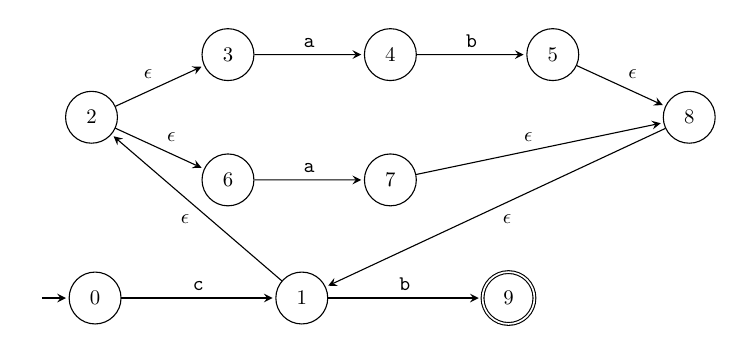
\begin{tikzpicture}[->,>=stealth,shorten >=1pt,auto,node distance=1.5 cm, scale = 0.75, transform shape,initial text={}]
  \node [initial,state] (99) {0};
  \node [state,right of= 99,xshift=2cm] (0) {1};
  \node [accepting,state,right of=0,xshift=2cm] (1) {9};
  \node [state,above left of=0,xshift=-2.5cm,yshift=2cm] (2) {2};
  \node [state,above right of=0,xshift=5.5cm,yshift=2cm] (3) {8};
  \node [state,below right of=2,xshift=1.25cm] (5) {6};
  \node [state,above right of=2,xshift=1.25cm] (6) {3};
  \node [state,right of=5,xshift=1.25cm] (7) {7};
  \node [state,right of=6,xshift=1.25cm] (8) {4};

  \node [state,right of=8,xshift=1.25cm] (97) {5};
  \path[->] (2) edge node {$\epsilon$} (5)
          edge node {$\epsilon$} (6)
        (5) edge node {{\tt a}} (7)
        (6) edge node {{\tt a}} (8)
        (7) edge node {$\epsilon$} (3)
        (8) edge node {{\tt b}} (97)
        (97) edge node {$\epsilon$} (3);

  \path[->] (0) edge node {{\tt b}} (1);
  \path[->] (3) edge node {$\epsilon$} (0);
  \path[->] (0) edge node {$\epsilon$} (2);
  \path[->] (99) edge node {{\tt c}} (0);
  \end{tikzpicture}
  \end{center}
  \caption{Figure of the NFA from the $E$ = {\tt c}({\tt ab}+{\tt a})$^*${\tt b}}
  \label{nfasimsucc}
\end{figure}
We now want to see if the input string {\tt caaabb} is accepted into N. The initial stateset \{$q^s\}=\{0\}$ \\
\begin{tabular}{l l l}
Simulate(N,{\tt caaabb}) & & \\
symbol {\tt c}: & $\epsilon$-$closure(\{0\})$ &$ = \{0\}$\\
&$reachable(\{0\},{\tt c})$& = $\{1\}$\\
symbol {\tt a}: & $\epsilon$-$closure(\{1\})$& = $\{1,2,3,6\}$\\
&$reachable(\{1,2,3,6\},{\tt a})$ & = $\{4,7\}$\\
symbol {\tt a}: & $\epsilon$-$closure(\{4,7\})$& = $\{1,2,3,4,6,7,8\}$\\
&$reachable(\{1,2,3,4,6,7,8\},{\tt a})$ &= $\{4,7\}$\\
symbol {\tt a}: & $\epsilon$-$closure(\{4,7\})$& = $\{1,2,3,4,6,7,8\}$\\
&$reachable(\{1,2,3,4,6,7,8\},{\tt a})$ &= $\{4,7\}$\\
symbol {\tt b}: & $\epsilon$-$closure(\{4,7\})$& = $\{1,2,3,4,6,7,8\}$\\
&$reachable(\{1,2,3,4,6,7,8\},{\tt b})$ &= $\{5,9\}$\\
symbol {\tt b}: & $\epsilon$-$closure(\{5,9\})$& = $\{1,2,3,5,6,8,9\}$\\
&$reachable(\{1,2,3,6,5,8,9\},{\tt b})$ &= $\{9\}$\\
\end{tabular}\\
After the final input symbol, it can be seen that the accepting state $q^a$ is in the final stateset. So the string caaabb is accepted in N.
\end{myex}
\begin{myex}
Using the NFA N from example \ref{simsuc} where $q^s=0$, the simulation attempts to check if string {\tt cabbbb} is accepted in N.\\
\begin{tabular}{l l l}
Simulate(N,{\tt cabbbb}) & & \\
symbol {\tt c}: & $\epsilon$-$closure(\{0\})$ &$ = \{0\}$\\
&$reachable(\{0\},{\tt c})$& = $\{1\}$\\
symbol {\tt a}: & $\epsilon$-$closure(\{1\})$& = $\{1,2,3,6\}$\\
&$reachable(\{1,2,3,6\},{\tt a})$ & = $\{4,7\}$\\
symbol {\tt b}: & $\epsilon$-$closure(\{4,7\})$& = $\{1,2,3,4,6,7,8\}$\\
&$reachable(\{1,2,3,4,6,7,8\},{\tt b})$ &= $\{5,9\}$\\
symbol {\tt b}: & $\epsilon$-$closure(\{5,9\})$& = $\{1,2,3,5,6,8,9\}$\\
&$reachable(\{1,2,3,6,5,8,9\},{\tt b})$ &= $\{9\}$\\
symbol {\tt b}: & $\epsilon$-$closure(\{9\})$& = $\{9\}$\\
&$reachable(\{9\},{\tt b})$ &= $\emptyset$\\
\end{tabular}\\
The $\emptyset$ is reached at the 5'th input symbol of {\tt cabbbb}, resulting in the simulation to fail. 
\end{myex}
\subsection{Tagged NFA}
Before introducing tagged NFA, we must define what a missmatch is. 
\begin{mydef}
A missmatch $M$ in a string $n$ with a alphabet $\Sigma$ is one of 3 types, insertion, deletion and alteration. An insertion is where a symbol in $\Sigma$ is added to $n$. A deletion is where a symbol in $n$ is removed. A alteration is where a symbol in $n$ is changed with a symbol in $\Sigma$. 
\end{mydef}
NFA's do not handle missmatching in strings per default, to introduce this, a new set of transitions is added to the NFA. This type of NFA is called a Tagged NFA. 
\begin{mydef}
A tagged NFA is a 6 tuple $(Q,\Sigma,\Delta,q^s,q^a,\Delta')$ where the first 5 elements is a standard NFA and $\Delta'$ is a set of 4 tuples containing $\epsilon$ transitions for missmatches. The type of $\Delta'$ is $\Delta' \subseteq Q ~x~ \{\epsilon\} ~x~ Q ~x~ M$.  
\end{mydef}

\subsection{Constructing TNFA}
TNFAs are constructed the same way as shown in tabel \ref{tab:NFA_TAB}, with the exception when constructing literals. A new set of $\epsilon$-transitions is added as shown in tabel \ref{tab:TNFA} as the new literal construction rule. The new transitions added in $\Delta'$ is shown as a red arrow which denotes a deletion transition, a green arrow for the insertion transition and a blue arrow for the alteration transition.
\begin{table}[h]\label{nfac}
\caption{Translating table for literal construction of TNFA}
\centering
\begin{tabular}{*{2}{m{0.4\textwidth}}}
\hline
\begin{center}$a$\end{center} &\begin{center}
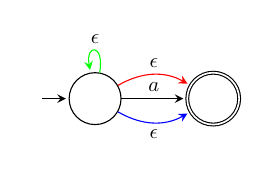
\begin{tikzpicture}[->,>=stealth,shorten >=1pt,auto,node distance=2 cm, scale = 0.75, transform shape,initial text={}]
  \node [initial, state] (0) {};
  \node [accepting,state, right of=0] (1) {};

  \path[->] (0) edge node [above] {$a$} (1);
  \path[->] (0) edge [color=green, in=100,out=80,loop] node [color=black, above] {$\epsilon$} (0);
  \path[->] (0) edge [color=red,bend left] node [color=black, above] {$\epsilon$} (1);

  \path[->] (0) edge [color=blue,bend right] node [color=black, below] {$\epsilon$} (1);
\end{tikzpicture}\end{center}\\
\hline
\end{tabular}
\label{tab:TNFA}
\end{table}



\newpage
\subsection{Simulating TNFA}\label{section_TNFA}
TNFA simulation adds an additional argument for the amount of mismatches allowed. The stateset contains 4 tuples of $(Q,i,d,a)$ where i,d and a is a count of how many of each transition has been used. The $\epsilon-closure$ and $reachable$ functions are extended to allow for for a set of 4 tuples.
\begin{mydef} 
Given a 4 tuple containing a state and mismatch counters $S(s,i,d,a)$, and a mismatch type $M$, the $t$-$reachable$ of S is a 4 tuple with the state that is reachable following the tagged transtion of the mismatch type $M$ in $\Delta'$ and the mismatch counters, with the mismatch type increased by one.  
\end{mydef}
\begin{algorithm}[h!]
  \caption{TNFA Simulation
    \label{tnfasim}}
  \begin{algorithmic}[1]
    \Require{$N$ is a TNFA and $s$ is a string, M is a 3-tuple of mismatches allowed}
    \Ensure{True if $s$ is accepted in $N$ with $M$ mismatches, False if $s$ is rejected in $N$}
    \Function{TNFA Simulation}{$N(Q,\Sigma,\Delta,q^s,q^a,\Delta'), s,M$}
      \Let{$stateset$}{$\{q^s,0,0,0\}$} 
      \For{{\bf each} symbol {\bf in} $s$}
        \If{$stateset = \emptyset$} 
            \State \Return{False}
        \EndIf
        \Let{$next$}{$\emptyset$}
        \Let{$states$}{$\epsilon$-closure($stateset$)}
        \Let{$next$}{$reachable(symbol,states)$}
        	\Let{$t\_next$}{$TNFA$-$reach(states,M)$}
          \Let{$stateset$}{$next \cup t\_next$}
      \EndFor
      \If{$q^a \in stateset$}
        \State \Return{True}
      \EndIf
      \State \Return{False}
    \EndFunction
  \end{algorithmic}
\end{algorithm}

\begin{algorithm}[h!]
  \caption{
    \label{tnfatrans}}
  \begin{algorithmic}[1]
    \Require{$states$ is a set of 4 tuples with a state q and mismatches occured, $M$  is a 3-tuple of mismatches allowed}
    \Ensure{A stateset with states that are reachable from $states$ using mismatches}
    \Function{$TNFA$-$reach$}{$states,M(ins,del,alt)$}
      \Let{$stateset$}{$\emptyset$} 
      \For{{\bf each} state(s,i,d,a) {\bf in} $states$}
        \Let{$stateset$}{$stateset \cup reachable(state)$}
        \If{$i < ins$}
        	\Let{$stateset$}{$stateset ~ \cup ~ (t$-$reachable(state,i))$}
        \EndIf
        \If{$d < del$}
        	\Let{$stateset$}{$stateset ~\cup ~ (t$-$reachable(state,d))$}
        \EndIf
        \If{$a < alt$}
        	\Let{$stateset$}{$stateset ~\cup~ (t$-$reachable(state,a))$}
        \EndIf
      \EndFor
      \State \Return{$stateset$}
    \EndFunction
  \end{algorithmic}
\end{algorithm}

\newpage


\begin{myex}
Given the RE $E= {\tt abc}^*{\tt d}$ the resulting TNFA N can be seen in Figure \ref{tnfa:simsuc}
\begin{figure}[H]
\begin{center}
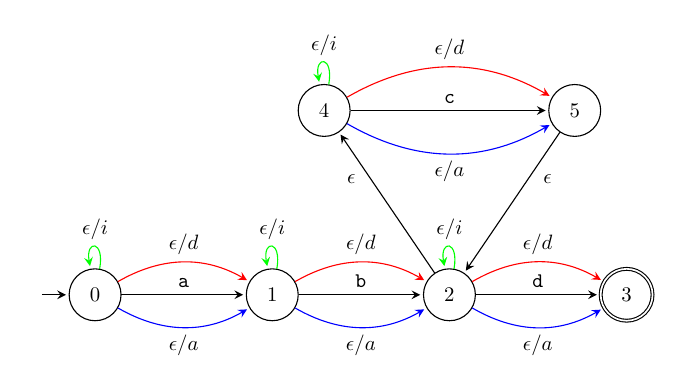
\begin{tikzpicture}[->,>=stealth,shorten >=1pt,auto,node distance=3 cm, scale = 0.75, transform shape,initial text={}]
  \node [initial, state] (0) {0};
  \node [state,right of=0] (1) {1};
  \node      [state,right of=1] (2) {2};
   \node     [accepting,state,right of=2] (3) {3};
    \node    [state,above left of=2,yshift=1cm] (4) {4};
    \node    [state,above right of=2,yshift=1cm] (5) {5};


   \path[->] (0) edge node {{\tt a}} (1)
         (1) edge node {{\tt b}} (2)
         (2) edge node {{\tt d}} (3)
           edge node [near end] {$\epsilon$} (4)
         (4) edge node {{\tt c}} (5)
         (5) edge node [near start] {$\epsilon$} (2);


  \path[->] (0) edge [color=green, in=100,out=80,loop] node [color=black, above] {$\epsilon/i$} (0);
  \path[->] (0) edge [color=red,bend left] node [color=black, above] {$\epsilon/d$} (1);
  \path[->] (0) edge [color=blue,bend right] node [color=black, below] {$\epsilon/a$} (1);


  \path[->] (1) edge [color=green, in=100,out=80,loop] node [color=black, above] {$\epsilon/i$} (1);
  \path[->] (1) edge [color=red,bend left] node [color=black, above] {$\epsilon/d$} (2);
  \path[->] (1) edge [color=blue,bend right] node [color=black, below] {$\epsilon/a$} (2);

  \path[->] (2) edge [color=green, in=100,out=80,loop] node [color=black, above] {$\epsilon/i$} (2);
  \path[->] (2) edge [color=red,bend left] node [color=black, above] {$\epsilon/d$} (3);
  \path[->] (2) edge [color=blue,bend right] node [color=black, below] {$\epsilon/a$} (3);

  \path[->] (4) edge [color=green, in=100,out=80,loop] node [color=black, above] {$\epsilon/i$} (4);
  \path[->] (4) edge [color=red,bend left] node [color=black, above] {$\epsilon/d$} (5);
  \path[->] (4) edge [color=blue,bend right] node [color=black, below] {$\epsilon/a$} (5);
\end{tikzpicture}
\end{center}
\caption{TNFA of expression $E = {\tt abc}^*{\tt d}$}
\label{tnfa:simsuc}
\end{figure}
We now want to see if the input string {\tt "abbdd"} is accepted in N allowing 1 insertion and 1 deletion. The initial stateset \{($q^s$,i,d,a)\} =\{(0,0,0,0)\}\\\\
\begin{table}[h!]
\small
\begin{tabular}{l l l}
\multicolumn{2}{l}{TNFASimulate(N,{\tt abbdd},(1,1,0)):}\\
symbol {\tt a}:& $\epsilon$-$closure$(\{(0,0,0,0)\})&=\{(0,0,0,0)\}\\
&$reachable$(\{(0,0,0,0)\},{\tt a})&=\{(1,0,0,0)\}\\
&$t$-$reachable$(\{(0,0,0,0)\},i)&=\{(0,1,0,0)\}\\
&$t$-$reachable$(\{(0,0,0,0)\},d)&=\{(1,0,1,0)\}\\
&$next\_stateset$&=\{(1,0,0,0),(0,1,0,0),(1,0,1,0)\}\\
\\
symbol {\tt b}:& $\epsilon$-$closure$(\{(1,0,0,0),(0,1,0,0),(1,0,1,0)\}) &=\{(1,0,0,0),(0,1,0,0),(1,0,1,0)\}\\
&$reachable$(\{(1,0,0,0),(0,1,0,0),(1,0,1,0)\},{\tt b})&=\{(2,0,0,0),(2,0,1,0)\}\\
&$t$-$reachable$(\{(1,0,0,0),(0,1,0,0),(1,0,1,0)\},i)&=\{(1,1,0,0),(1,1,1,0)\}\\
&$t$-$reachable$(\{(1,0,0,0),(0,1,0,0),(1,0,1,0)\},d)&=\{(2,0,1,0),(1,1,1,0)\}\\
&$next\_stateset$&=\{(2,0,0,0),(2,0,1,0),(1,1,0,0),(1,1,1,0)\}\\
\\ 
symbol {\tt b}:&$\epsilon$-$closure$(\{(2,0,0,0),(2,0,1,0),(1,1,0,0),(1,1,1,0)\})&=\{(2,0,0,0),(2,0,1,0),(1,1,0,0)\\
&&~~~,(1,1,1,0),(4,0,0,0),(4,0,1,0)\}\\
&$reachable$(\{(2,0,0,0),(2,0,1,0),(1,1,0,0),(1,1,1,0)&=\{(2,1,0,0),(2,1,1,0)\}\\
&~~~~~~~~~~~~~~,(4,0,0,0),(4,0,1,0)\},{\tt b})\\

&$t$-$reachable$(\{(2,0,0,0),(2,0,1,0),(1,1,0,0),(1,1,1,0)&=\{(2,1,0,0),(2,1,1,0),(4,1,0,0),(4,1,1,0)\}\\
&~~~~~~~~~~~~~~~~,(4,0,0,0),(4,0,1,0)\},i)\\

&$t$-$reachable$(\{(2,0,0,0),(2,0,1,0),(1,1,0,0),(1,1,1,0)&=\{(3,0,1,0),(3,1,1,0),(5,0,1,0)\}\\
&~~~~~~~~~~~~~~~~,(4,0,0,0),(4,0,1,0)\},d)\\

&$next\_stateset$&=\{(2,1,0,0),(2,1,1,0),(3,0,1,0),(3,1,1,0)\\
&&~~~,(4,1,0,0),(4,1,1,0),(5,0,1,0)\}\\
\\
symbol {\tt d}:&$\epsilon$-$closure$(\{(2,1,0,0),(2,1,1,0),(3,0,1,0),(3,1,1,0)&=\{(2,1,0,0),(2,0,1,0),(2,1,1,0),(3,0,1,0),(3,1,1,0)\\
&~~~~~~~~~~~~~~,(4,1,0,0),(4,1,1,0),(5,0,1,0)\}&~~~,(4,1,0,0),(4,0,1,0),(4,1,1,0),(5,0,1,0)\}\\
&$reachable$(\{(2,1,0,0),(2,0,1,0),(2,1,1,0),(3,0,1,0),(3,1,1,0)&=\{(3,1,0,0),(3,0,1,0),(3,1,1,0)\}\\
&~~~~~~~~~~~~~~,(4,1,0,0),(4,0,1,0),(4,1,1,0),(5,0,1,0)\},{\tt d})\\

&$t$-$reachable$(\{(2,1,0,0),(2,0,1,0),(2,1,1,0),(3,0,1,0),(3,1,1,0)&=\{(3,1,1,0),(5,1,1,0)\}\\
&~~~~~~~~~~~~~~~~,(4,1,0,0),(4,0,1,0),(4,1,1,0),(5,0,1,0)\},i)\\

&$t$-$reachable$(\{(2,1,0,0),(2,0,1,0),(2,1,1,0),(3,0,1,0),(3,1,1,0)&=\{(3,1,1,0),(5,1,1,0)\}\\
&~~~~~~~~~~~~~~~~,(4,1,0,0),(4,0,1,0),(4,1,1,0),(5,0,1,0)\},d)\\
&$next\_stateset$&=\{(3,1,0,0),(3,0,1,0),(3,1,1,0),(5,1,1,0)\}\\
\\
symbol {\tt d}:&$\epsilon$-$closure$(\{(3,1,0,0),(3,0,1,0),(3,1,1,0),(5,1,1,0)\})&=\{(3,1,0,0),(3,0,1,0),(3,1,1,0),(5,1,1,0)\\
&&~~~,(2,1,1,0),(4,1,1,0)\}\\
&$reachable$(\{(3,1,0,0),(3,0,1,0),(3,1,1,0),(5,1,1,0)&=\{3,1,1,0\}\\
&~~~~~~~~~~~~~~,(2,1,1,0),(4,1,1,0)\},{\tt d})\\
&$t$-$reachable$(\{(3,1,0,0),(3,0,1,0),(3,1,1,0),(5,1,1,0)&=$\emptyset$\\
&~~~~~~~~~~~~~,(2,1,1,0),(4,1,1,0)\},i)\\
&$t$-$reachable$(\{(3,1,0,0),(3,0,1,0),(3,1,1,0),(5,1,1,0)&=$\emptyset$\\
&~~~~~~~~~~~~~,(2,1,1,0),(4,1,1,0)\},d)\\
&$final\_stateset$&=\{3,1,1,0\}
\end{tabular}
\end{table}\\
The string {\tt "abbdd"} is accepted, since $q^a\in final\_stateset$, which have 1 insertion and 1 deletion.
\end{myex}
\begin{myex}
Given the RE $E={\tt abbca}$ the TNFA $N$ of $E$ is seen in Figure \ref{tnfa:simfail}.
\begin{figure}[h!]
\begin{center}
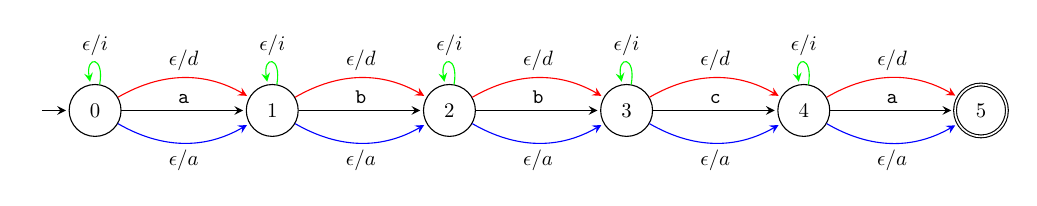
\begin{tikzpicture}[->,>=stealth,shorten >=1pt,auto,node distance=3 cm, scale = 0.75, transform shape,initial text={}]
  \node [initial, state] (0) {0};
  \node [state,right of=0] (1) {1};
  \node      [state,right of=1] (2) {2};
   \node     [state,right of=2] (3) {3};
   \node     [state,right of=3] (4) {4};
   \node     [accepting,state,right of=4] (5) {5};


   \path[->] (0) edge node {{\tt a}} (1)
         (1) edge node {{\tt b}} (2)
         (2) edge node {{\tt b}} (3)
         (3) edge node {{\tt c}} (4)
         (4) edge node {{\tt a}} (5);


  \path[->] (0) edge [color=green, in=100,out=80,loop] node [color=black, above] {$\epsilon/i$} (0);
  \path[->] (0) edge [color=red,bend left] node [color=black, above] {$\epsilon/d$} (1);
  \path[->] (0) edge [color=blue,bend right] node [color=black, below] {$\epsilon/a$} (1);


  \path[->] (1) edge [color=green, in=100,out=80,loop] node [color=black, above] {$\epsilon/i$} (1);
  \path[->] (1) edge [color=red,bend left] node [color=black, above] {$\epsilon/d$} (2);
  \path[->] (1) edge [color=blue,bend right] node [color=black, below] {$\epsilon/a$} (2);

  \path[->] (2) edge [color=green, in=100,out=80,loop] node [color=black, above] {$\epsilon/i$} (2);
  \path[->] (2) edge [color=red,bend left] node [color=black, above] {$\epsilon/d$} (3);
  \path[->] (2) edge [color=blue,bend right] node [color=black, below] {$\epsilon/a$} (3);

  \path[->] (3) edge [color=green, in=100,out=80,loop] node [color=black, above] {$\epsilon/i$} (3);
  \path[->] (3) edge [color=red,bend left] node [color=black, above] {$\epsilon/d$} (4);
  \path[->] (3) edge [color=blue,bend right] node [color=black, below] {$\epsilon/a$} (4);

  \path[->] (4) edge [color=green, in=100,out=80,loop] node [color=black, above] {$\epsilon/i$} (4);
  \path[->] (4) edge [color=red,bend left] node [color=black, above] {$\epsilon/d$} (5);
  \path[->] (4) edge [color=blue,bend right] node [color=black, below] {$\epsilon/a$} (5);
\end{tikzpicture}
\end{center}
\caption{TNFA of expression $E = {\tt abbca}$}
\label{tnfa:simfail}
\end{figure}
We now want to see the string {\tt "abccec"} is accepted into $N$ given the initial stateset \{(0,0,0,0)\} and allowing 1 insertion and 1 alternation.\\
\begin{table}[h!]
\small
\begin{tabular}{l l l}
\multicolumn{2}{l}{TNFASimulate(N,{\tt abccec},(1,0,1)):}\\
symbol {\tt a}:& $\epsilon$-$closure$(\{(0,0,0,0)\})&=\{(0,0,0,0)\}\\
&$reachable$(\{(0,0,0,0)\},{\tt a})&=\{(1,0,0,0)\}\\
&$t$-$reachable$(\{(0,0,0,0)\},i)&=\{(0,1,0,0)\}\\
&$t$-$reachable$(\{(0,0,0,0)\},a)&=\{(1,0,0,1)\}\\
&$next\_stateset$&=\{(1,0,0,0),(0,1,0,0),(1,0,0,1)\}\\
\\
symbol {\tt b}:& $\epsilon$-$closure$(\{(1,0,0,0),(0,1,0,0),(1,0,0,1)\})&=\{(1,0,0,0),(0,1,0,0),(1,0,0,1)\}\\
&$reachable$(\{(1,0,0,0),(0,1,0,0),(1,0,0,1)\},{\tt b})&=\{(2,0,0,0),(2,0,0,1)\}\\
&$t$-$reachable$(\{(1,0,0,0),(0,1,0,0),(1,0,0,1)\},i)&=\{(1,1,0,0),(1,1,0,1)\}\\
&$t$-$reachable$(\{(1,0,0,0),(0,1,0,0),(1,0,0,1)\},a)&=\{(1,1,0,1),(2,0,0,1)\}\\
&$next\_stateset$&=\{(1,1,0,0),(1,1,0,1),(2,0,0,0),(2,0,0,1)\}\\
\\
symbol {\tt c}:& $\epsilon$-$closure$(\{(1,1,0,0),(1,1,0,1),(2,0,0,0),(2,0,0,1)\})&=\{(1,1,0,0),(1,1,0,1),(2,0,0,0),(2,0,0,1)\}\\
&$reachable$(\{(1,1,0,0),(1,1,0,1),(2,0,0,0),(2,0,0,1)\},{\tt c})&=$\emptyset$\\
&$t$-$reachable$(\{(1,1,0,0),(1,1,0,1),(2,0,0,0),(2,0,0,1)\},i)&=\{(2,1,0,0),(2,1,0,1)\}\\
&$t$-$reachable$(\{(1,1,0,0),(1,1,0,1),(2,0,0,0),(2,0,0,1)\},a)&=\{(2,1,0,1),(3,0,0,1)\}\\
&$next\_stateset$&=\{(2,1,0,0),(2,1,0,1),(3,0,0,1)\}\\
\\
symbol {\tt c}:& $\epsilon$-$closure$(\{(2,1,0,0),(2,1,0,1),(3,0,0,1)\})&=\{(2,1,0,0),(2,1,0,1),(3,0,0,1)\}\\
&$reachable$(\{(2,1,0,0),(2,1,0,1),(3,0,0,1)\},{\tt c})&=\{(4,0,0,1)\}\\
&$t$-$reachable$(\{(2,1,0,0),(2,1,0,1),(3,0,0,1)\},i)&=\{(3,1,0,1)\}\\
&$t$-$reachable$(\{(2,1,0,0),(2,1,0,1),(3,0,0,1)\},a)&=\{(3,1,0,1)\}\\
&$next\_stateset$&=\{(3,1,0,1),(4,0,0,1)\}\\
\\
symbol {\tt e}:& $\epsilon$-$closure$(\{(3,1,0,1),(4,0,0,1)\})&=\{(3,1,0,1),(4,0,0,1)\}\\
&$reachable$(\{(3,1,0,1),(4,0,0,1)\},{\tt e})&=$\emptyset$\\
&$t$-$reachable$(\{(3,1,0,1),(4,0,0,1)\},i)&=\{(4,1,0,1)\}\\
&$t$-$reachable$(\{(3,1,0,1),(4,0,0,1)\},a)&=$\emptyset$\\
&$next\_stateset$&=\{(4,1,0,1)\}\\
\\
symbol {\tt c}:& $\epsilon$-$closure$(\{(4,1,0,1)\})&=\{(4,1,0,1)\}\\
&$reachable$(\{(4,1,0,1)\},{\tt c})&=$\emptyset$\\
&$t$-$reachable$(\{(4,1,0,1)\},i)&=$\emptyset$\\
&$t$-$reachable$(\{(4,1,0,1)\},a)&=$\emptyset$\\
&$next\_stateset$&=$\emptyset$\\
\\
\end{tabular}
\end{table}\\\\\\
At the end of reading input $\emptyset$ is found, the string {\tt abccec} is not accepted into $N$.
\end{myex}
%Simulation of NFA

\section{Scan\_For\_Matches}\label{scanformatches}
Scan\_for\_matches is a string-searching tool created by Ross Overbeek, David 
Joerg and Morgan Price in C which searches through text files. Users specify 
what they want to search for by defining a pattern, and scan\_for\_matches 
returns all matches that corresponds to the specified pattern. 
\begin{mydef}\label{patex}
Let $\Sigma$ denote an alphabet. Then we can define a pattern unit as follows:\\
\begin{tabular}{|r|l|}
\hline
{\tt h}&Match the sequence h, where $h\in\Sigma*$\\
\hline
{\tt n...m}&Match n to m characters where n $\leq$ m\\
\hline
{\tt x=n...m}&Match n to m characters, and call the sequence x\\
\hline
{\tt x $|$ y}&Match either pattern x or pattern y\\
\hline
{\tt x[n,m,l]}&\pbox{20cm}{Match pattern x, allowing for n mismatches, m deletions and insertions\\ where n,m,l $\geq$ 0}\\
\hline
{\tt length(x+y) $<$ n}&The length of patterns x+y$<$n where n $>$ 0\\
\hline
{\tt z=\{uv, vu\}}&\pbox{20cm}{Create a pattern rule where u is the complement of v, and v is the\\ complement of u,
                               where $u,~v\in\Sigma$, and call the rule z}\\
\hline
{\tt $<$x}&Match the reverse of pattern x\\
\hline
{\tt $\sim$x}&\pbox{20cm}{Match the reverse complement of pattern x using the G-C, \\C-G, A-T and T-A pairing rule}\\
\hline
{\tt z$\sim$x}&\pbox{20cm}{Match the reverse complement of pattern x using pattern rule z}\\
\hline
{\tt \textasciicircum ~x}&\pbox{20cm}{Match only pattern x if it is at the start of a string}\\
\hline
{\tt x \$}&Match only pattern x if it is at the end of a string\\
\hline
\end{tabular}
\end{mydef}

\begin{mydef}\label{patc}
Let $\Lambda$ be any pattern unit in definition~\ref{patex}. Let ${\tt E}\in\Lambda$.
Let {\tt 0} be the empty string. Let A be a pattern that we are processing.
A pattern may then be constructed as such: 
\begin{align*}
{\tt A~} &{\tt =~A'~A~|~0}\\
{\tt A'~} &{\tt=~E}
\end{align*}
\end{mydef}
Definition~\ref{patc} states that a pattern may be any combination of the pattern 
units defined in definition~\ref{patex}.
\begin{mydef}\label{patlint}
Let $\Sigma$ be an alphabet. Let {\tt a$\in\Sigma$}. Let {\tt 0} be the empty 
string.
Then the language interpretation of definition~\ref{patex} is defined as follows:
\begin{align*}
L({\tt 0})~&=~\emptyset\\
L({\tt a})~&=~\{{\tt a}\}\\
L({\tt n...n})~&=~\underbrace{L({\tt a})L({\tt a})...L({\tt a})}_\text{n}\\
L({\tt n...m})~&=~L({\tt n...n})\cup L({\tt n+1...n+1})\cup...\cup L({\tt m-1...m-1})\cup L({\tt m...m})~=~\bigcup\limits_{n={\tt n}}^{\tt m} L(n...n)\\
L({\tt E_1~E_2})~&=L({\tt E_1})~L({\tt E_2})\\
L({\tt E_1~|~E_2})~&=~L({\tt E}_{\tt 1})~\cup~L({\tt E}_{\tt 2})\\
L({\tt {\sim}E})~&=~{\sim}L({\tt E})\\
L({\tt <E})~&=~<L({\tt E})\\
L({\tt length(E_ 1 )+ E_2} )~&=~{\tt length(}L({\tt E_1}){\tt+} L({\tt E_2 )})\\
L({\tt E_1{\sim}E_2}~&=~L({\tt E_1}){\sim}L({\tt E_2})\\
L({\tt~\hat{}~E})~&=~\hat{} L({\tt E})\\
L({\tt E~\$})~&=~L({\tt E})~\$
\end{align*}
\end{mydef}
Definition~\ref{patlint} depicts the language interpretation of scan\_for\_matches.
The language interpretation have some functionality that can't properly be 
shown in a language interpretation, like the modifier $<$. This is because 
a regular language does not support the reverse of a match. 
\\Below are examples of scan\_for\_matches patterns.
\begin{myex}\label{stemex}
Say we want to write a pattern that finds the sequence {\tt GUUC}, allowing 
one mismatch, followed by a random sequence which has a length between 3 and 5, 
followed by the reverse complement of the first sequence that we found. We can 
then write this as \begin{center}
{\tt p1=GUUC[1,0,0] 3...5 \textasciitilde p1}
\end{center}
\end{myex}
Example \ref{stemex} will match a stem loop as described in section 
\ref{structs}. Note that if we wanted to find all stem loops in a file where 
the bonded bases are of length 
4, we would replace {\tt GUUC[1,0,0]} with an arbitrary sequence of characters 
by writing {\tt p1=4..4 3..5 \textasciitilde p1}. 

%implementation
%\section{Method}
%\newpage
\section{TRE}\label{tre}
  
For our implementation of scan\_for\_matches patterns in TRE, we needed to 
first make a brief analysis of the program to see what it could and couldn't 
do. What we discovered after our initial tests was that TRE defined each 
new line as a delimiter (a delimiter defines at which points the text will be 
separated, so each chunk can be evaluated individually). 
This caused a small, but surmountable, problem; chromosome data 
should be read as one continous line that spans over many lines. Since TRE 
split the data up per line, if a match spanned over more than one line, it 
wouldn't find it. To this problem there was an easy fix; we would make a small 
wrapper which would feed the text file to TRE, removing any newlines as they 
occurred.\\
With this problem solved, we did a trial test to check the accuracy and 
running time of TRE. Here we encountered a second, greater problem; TRE 
would find only one match per delimiter (the first longest match with fewest 
errors, prioritizing exact matches). This was a harder problem to fix, because this feature was 
deeply entrenched in the code, and everything had seemingly been designed 
around this feature. The searching tool that TRE uses, agrep, only receives 
the best match that the other tools of TRE has found, but throughout TRE's 
code, it won't save the matches it has found, but instead repeatedly discard old 
matches. The problem is compounded by the fact that TRE will immediately stop searching the 
text if it finds an exact match, leaving behind potential matches. In light of 
these problems, we decided that attempting to fully understand TRE's design and 
subsequently heavily modding it in order for it to return all matches would 
take too long, and that we would instead create our own solution.

\newpage
\section{Our Implementation}
Having defined an algorithm in Section~\ref{sec:tnfa}, we wished to construct a simple program based on TNFA, which would pattern-match data allowing for mismatches.

When wrote a simple program in C++ which we named TNFA Pattern-Matcher (TPaMa). TPaMa is able to create a TNFA from a RE, and it supports a series of RE symbols, including $+, ^*, |, ?$ along with concatenation of characters. An example of a TFNA from a RE could be RE "(GAT)+" which would produce a structure as shown in Figure~\ref{fig:gat}

\begin{figure}[h!]
\centering
\includegraphics[width=0.5\textwidth]{lib/gat.png}
\caption{Example of how TPaMa constructs a TNFA from RE (GAT)+}
\label{fig:gat}
\end{figure}

However, currently the search implementation of TPaMa only support simple patterns such as "GAT" which does not cause any $\epsilon$-transitions to be constructed, this choice was made so we could focus on the performance of mismatching while giving support to the most crucial part of pattern-matching.

This also meant that determining reachable states, as mentioned in Algorithm~\ref{tnfasim} \&~\ref{tnfatrans} is rather straightforward, as there's only up to one possible next state for every state (zero for the final state).

To handle mismatching, recall Table~\ref{nfac}:

%\begin{table}[h]
\begin{tabular}{*{2}{m{0.4\textwidth}}}
\begin{center}$a$\end{center} &\begin{center}
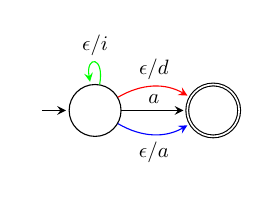
\begin{tikzpicture}[->,>=stealth,shorten >=1pt,auto,node distance=2 cm, scale = 0.75, transform shape,initial text={}]
  \node [initial, state] (0) {};
  \node [accepting,state, right of=0] (1) {};

  \path[->] (0) edge node [above] {$a$} (1);
  \path[->] (0) edge [color=green, in=100,out=80,loop] node [color=black, above] {$\epsilon/i$} (0);
  \path[->] (0) edge [color=red,bend left] node [color=black, above] {$\epsilon/d$} (1);

  \path[->] (0) edge [color=blue,bend right] node [color=black, below] {$\epsilon/a$} (1);
\end{tikzpicture}\end{center}\\
\end{tabular}
%\end{table}

There's three different types of mismatches. Instead of having three types of transitions we simulate this by having three counters in each state, one for each type of mismatch (insertions, alternation and deletion), keeping track of the remaining number of mismatches allowed in the match. Whenever a match can not be made, for each mismatch counter with a positive value, a new state is created.


\begin{lstlisting}[language=C++]
if((*it).insertions > 0){
    add_state(it, (*it).node, (*it).path+1, (*it).insertions-1, (*it).deletions, 
        (*it).mutations);
    ++it;
}
if((*it).mutations > 0){
    add_state(it, (*it).node->next, (*it).path+1, (*it).insertions, (*it).deletions,
        (*it).mutations-1);
    ++it;
}
 if((*it).deletions > 0){
    add_state(it, (*it).node->next, (*it).path, (*it).insertions, (*it).deletions-1,
        (*it).mutations);
    ++it;
}
\end{lstlisting}


\section{Results}
\begin{table}[h!]
\begin{tabular}{ c | c | c |  c | c | c | c |  c | c | c |  c }
 ~chr1.fa & ~chr2.fa  & ~chr3.fa & ~chr4.fa & ~chr5.fa & ~chr6.fa &  ~chr7.fa & ~chr8.fa & ~chr9.fa & chr10.fa & chr11.fa \\
 \hline
246.284 & 242.003 & 198.723 & 190.526 & 180.152 & 170.233 & 158.202 & 145.704 & 139.726 & 134.846 & 133.928
\end{tabular}
\begin{tabular}{ c | c | c |  c | c | c | c |  c | c | c |  c }
chr12.fa & chr13.fa & chr14.fa & chr15.fa & chr16.fa & chr17.fa & chr18.fa & chr19.fa & chr20.fa & chr21.fa & chr22.fa\\
\hline
131.833 & 113.698 & 105.954 & 99.947 & 88.481 & 78.468 & 75.820 & 63.563 & 62.193 & 46.761 & 49.498
\end{tabular}
\caption{Fasta files from http://hgdownload.cse.ucsc.edu/goldenPath/hg18/chromosomes/ with sizes in KB}
\label{tab:sizes}
\end{table}
Looking at Table~\ref{tab:sizes}, we have a series of fasta files, ranging from 246.284KB to 46.761 KB in size, each fasta file has a number, and besides $chr22.fa$, every number is decreasingly lower in size as to the previous.

\begin{figure}[h!]
\centering
\includegraphics[width=0.6\textwidth]{Benchmarking/1ins.png}
\caption{Running time of search through fasta files mentioned in Table~\ref{tab:sizes},  allowing one insertions on pattern TGCAAGCGTTAAT}
\end{figure}

\begin{figure}[h!]
\centering
\includegraphics[width=0.6\textwidth]{Benchmarking/2ins.png}
\caption{Running time of search through fasta files mentioned in Table~\ref{tab:sizes},  allowing two insertions on pattern TGCAAGCGTTAAT}
\end{figure}


%alternative soloutions
\section{Alternative soloutions}
\subsection{Forming patterns using Regular expressions}
The initial goal of this project was to use regular expressions to match the sequences. The problem of only using regular expressions, is the amount of patterns explode in size when adding mismatching. Following is a description of how many patterns are formed from a pattern of length $n$. When a new pattern is formed, it constructs them into 1 regular expression using the alternation operator separating each of the new expressions. 

Mutations are done by having a character replaced by a wildcard. This is done for every character in the pattern. When adding multiple mutations, characters which are already wildcards are not changed. The formula for the amount of patterns formed from mutations is the number of combinations that can be formed from the amount of mutations in $t$. This is the binomial coefficient\footnote{\url{http://en.wikipedia.org/wiki/Binomial_coefficient}}. 

An insertion is a wildcard added between the characters in the pattern, so for each pattern $n-1$ new patterns occur.

A deletion is removing a character from the pattern. It is not allowed to remove a character next to an insertion, as this cannot occur in RNA and DNA strings. Given multiple insertions, they will be spread out throughout the pattern in most cases, so an approximation of how many patterns formed would be $(n - insertions * 2)$.

The final formula looks like ${n \choose m}*(n-1)*(n-i*2)$, where $n$ is the length of the string, $m$ is amount of mutations and i is amount of insertions.

\begin{myex}\label{altreg}
Given a pattern of size 30, with 2 mutations, 1 deletion, 1 insertion. It would produce the following amount of patterns: \\
\begin{center}
\text{After mutation:} $~{30 \choose 2} = 435$\\
\text{After insertion:} $435 * (30-1) = 12615$\\
After~Deletion:~$12615*(30-2) = 353220$
\end{center}
\end{myex}

As shown in example \ref{altreg}, the amount of patterns formed from using regular expressions could be too large for a regular expression matcher to find in a reasonable time. 

\section{Summary \& Future Work}
We presented an alternative type of NFA in Section \ref{section_TNFA}.
The alternation allowed for insertions, deletions and mutations when matching a pattern.
A runtime analysis showed that the new NFA type caused an increase in states which would grow as the errors were increased.
Future work would consist of preventing said growth, by making sure states which does repeated work are handled as a single state. 
Further work would extent on the TNFA to support more SFM features, and backreferenceing. 

Further more a research into preproccesing using suffix trees\footnote{\url{http://en.wikipedia.org/wiki/Suffix_tree}} could allow posible decrease in runtime.


% READ ME!!!!!!!
% Det der står i scan-for-matches omtaler et alfabet og et sprog, dette er først beskrevet i Theory/re.tex, derfor skal det ind bagefter
% HVIS vi skal beskrive scan-for-matches først, kan vi nævne at det findes et værktøj, og hvad det bruges til, men den måde det står beskrevet pt, funker ikke.
%related works, SFM TRE
% \READ ME
%\section{Method}
%
%experimental results
%\section{Conclusion}
\newpage
\nocite{*}
\bibliographystyle{unsrt}
\bibliography{./References/references}
\end{document}
